\documentclass[10pt]{beamer}

\mode<presentation> {
\usetheme{Goettingen}
}
\usepackage{tikz}
\usepackage[english]{babel}
\usepackage[latin1]{inputenc}
\usepackage[T1]{fontenc}
\usepackage{graphicx} 
\usepackage{tikz}
\usepackage{booktabs} 
\usepackage{amsmath}
\usepackage{url,color}
\usepackage{subfigure}
\usepackage{graphicx}
\usepackage{xcolor}
\usepackage{soul}
\usepackage{listings,,lstautogobble}
\usepackage{amsthm,amsfonts,amssymb,amscd,amsxtra}
\lstset{language=Java,
	keywordstyle=\color{RoyalBlue},
	basicstyle=\scriptsize\ttfamily,
	commentstyle=\ttfamily\itshape\color{gray},
	stringstyle=\ttfamily,
	showstringspaces=false,
	breaklines=true,
	frameround=ffff,
	frame=single,
	rulecolor=\color{black},
	autogobble=true
}
\usepackage{biblatex}
\addbibresource{references.bib}

\newcommand\myscalefactor{0.5}

\title[Proposal Review]{Control and Decision Making \\ in Systems Biology} 

\author{Northeastern University} 
\medskip

\date{December 13, 2021} 

\begin{document}

\begin{frame}
	\maketitle
	\small \hspace{3cm}
	{\begin{tabular}{r@{}l}
			Presenter: \ & Mahdiar Sadeghi \\
			Advisor:   \  & Prof. Eduardo Sontag \\
			Committee: \  & Dr. Irina Kareva \\
			& Prof. Mark Niedre \\
			& Prof. Carey Rappaport \\
			& Prof. Bahram Shafai
		\end{tabular}
	}
\end{frame}

%-------------------------------------------------%
\section{Outline}

\begin{frame}{Presentation outline}
	\vspace{15pt}
    \begin{enumerate}
    	\item Background
    	\item Chemotherapy
    	\item Immunotherapy
    	\item Epidemics
    	\item Acknowledgement
    \end{enumerate}
\end{frame}

%-------------------------------------------------%
\section{Background}

\begin{frame}{Practice and theory}
	Practice and theory in engineering and scientific research. The focus is to use modeling to make predictions outside previous experimental settings to come of with a better control/decision. \\
	\vspace{0.5cm}
		  \hspace{1cm}
		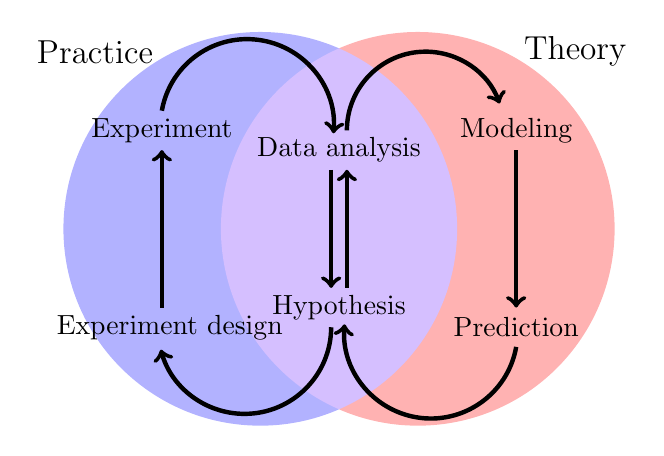
\begin{tikzpicture}
			\pgftransformscale{\myscalefactor}
			\begin{scope}[blend group = soft light]
				\fill[blue!30!white] (-2,0) ellipse (5 and 5);
				\fill[red!30!white]  (+2,0) ellipse (5 and 5);
			\end{scope}
			\draw[ultra thick, ->] (0.2,2.5) arc (0:-160:-2);
			\draw[ultra thick, ->] (-4.5,+3) arc (-10:-185:-2.2);
			\draw[ultra thick, ->] (-0.2,-2.5) arc (0:-165:+2.2);
			\draw[ultra thick, ->] (4.5,-3) arc (-10:-185:2.2);
			\draw [ultra thick, ->] (-0.2,+1.5) -- (-0.2,-1.5);
			\draw [ultra thick, ->] (+0.2,-1.5) -- (+0.2,+1.5);
			\draw [ultra thick, ->] (4.5,+2) -- (4.5,-2);
			\draw [ultra thick, ->] (-4.5,-2) -- (-4.5,+2);
			\node at (0,+2) {Data analysis};
			\node at (4.5,+2.5)  {Modeling};
			\node at (4.5,-2.5)  {Prediction};
			\node at (0,-2)  {Hypothesis};
			\node at (-4.5,+2.5)  {Experiment};
			\node at (-4.3,-2.5) {Experiment design};
			\node at (-6.2,4.5)[font=\large]    {Practice};
			\node at (+6,4.5)[font=\large]    {Theory};
		\end{tikzpicture}
\end{frame}

%-------------------------------------------------%
\section{Chemotherapy}

\begin{frame}{Cyclophosphamide: innate immune cell recriutment and tumor regression}
	The current standard of care limits the regiments used primaritly to daily dose and maximum-tolerated dose (MTD) treatments.
	\vspace{1cm}
	\begin{itemize}
		\item Motivation: Metronomic/intermittent experiments~\footfullcite{wu2014metronomic} in mice. A lower dose with a higher frequency than MTD were shown to reqruit immune system and reduce the tumor volume.
		\vspace{0.5cm}
		\item Objective: Use optimal control techniques in order to have a better treatment outcome among all possible dosing strategies.
	\end{itemize}
\end{frame}

\begin{frame}{Optimal control techniques for cancer treatment}
	Early efforts in using optimal control techniques for cancer treatment started in the 1970s for Radiotherapy~\footfullcite{bahrami1975optimal} and Chemotherapy~\footfullcite{swan1977optimal}. \\
	\vspace{0.5cm}
	Now, a new generation of quantitative experiments made it possible to have more realistic models of the system. \\
	\vspace{0.5cm}
	The goal is to use optimal control techniques to find a mathematically derived optimal regimen (MDOR) to be tested in a similar experimental settings.
\end{frame}

\subsection{Model}
\begin{frame}{A dynamic model for chemotherapy}
\small
\begin{subequations} \label{eq:chemo1}
	\begin{align} 
		\dot{T}(t) &=  k_{a} T(t) - \frac{k_{b}C(t)T(t)}{k_{c}C(t)+T(t)} - k_{d}T(t)I(t),\\
		\dot{I}(t) &= q X(t) -k_{e}T(t)I(t)-k_{f}C(t)I(t)-k_{g}Y(t)I(t)-k_{h}I,\\
		\dot{X}(t) &= \frac{q C(t)T(t)}{k_{i}C(t)+T(t)}-k_{j}X(t)-k_{k}X(t)Y(t),\\
		\dot{Y}(t) &= \frac{I(t)}{k_l+I(t)} - k_{m}Y(t) C(t),\\
		\dot{C}{t} &= u(t) - \frac{k_1 C(t)}{k_2 + C(t)}.
	\end{align}
\end{subequations}
Where Tumor $T$ represents the tumor volume, and the phenamenological variables immune system $I$, immunostimulatory $X$, immunossuppressor $Y$, and drug $C$ represent the dynamics in the tumor microenvinronment. \\
Model is fitted to the tumor and immune data in mouse experiments.
\end{frame}

%\begin{frame}{Steady-states of the model}
%	
%\end{frame}

\subsection{Metronomic}
\begin{frame}{Efficacy of metronomic regimens}
	140 mg/kg every 6 days as an optimal metronomic regimen. \\ \vspace{0.5cm}
	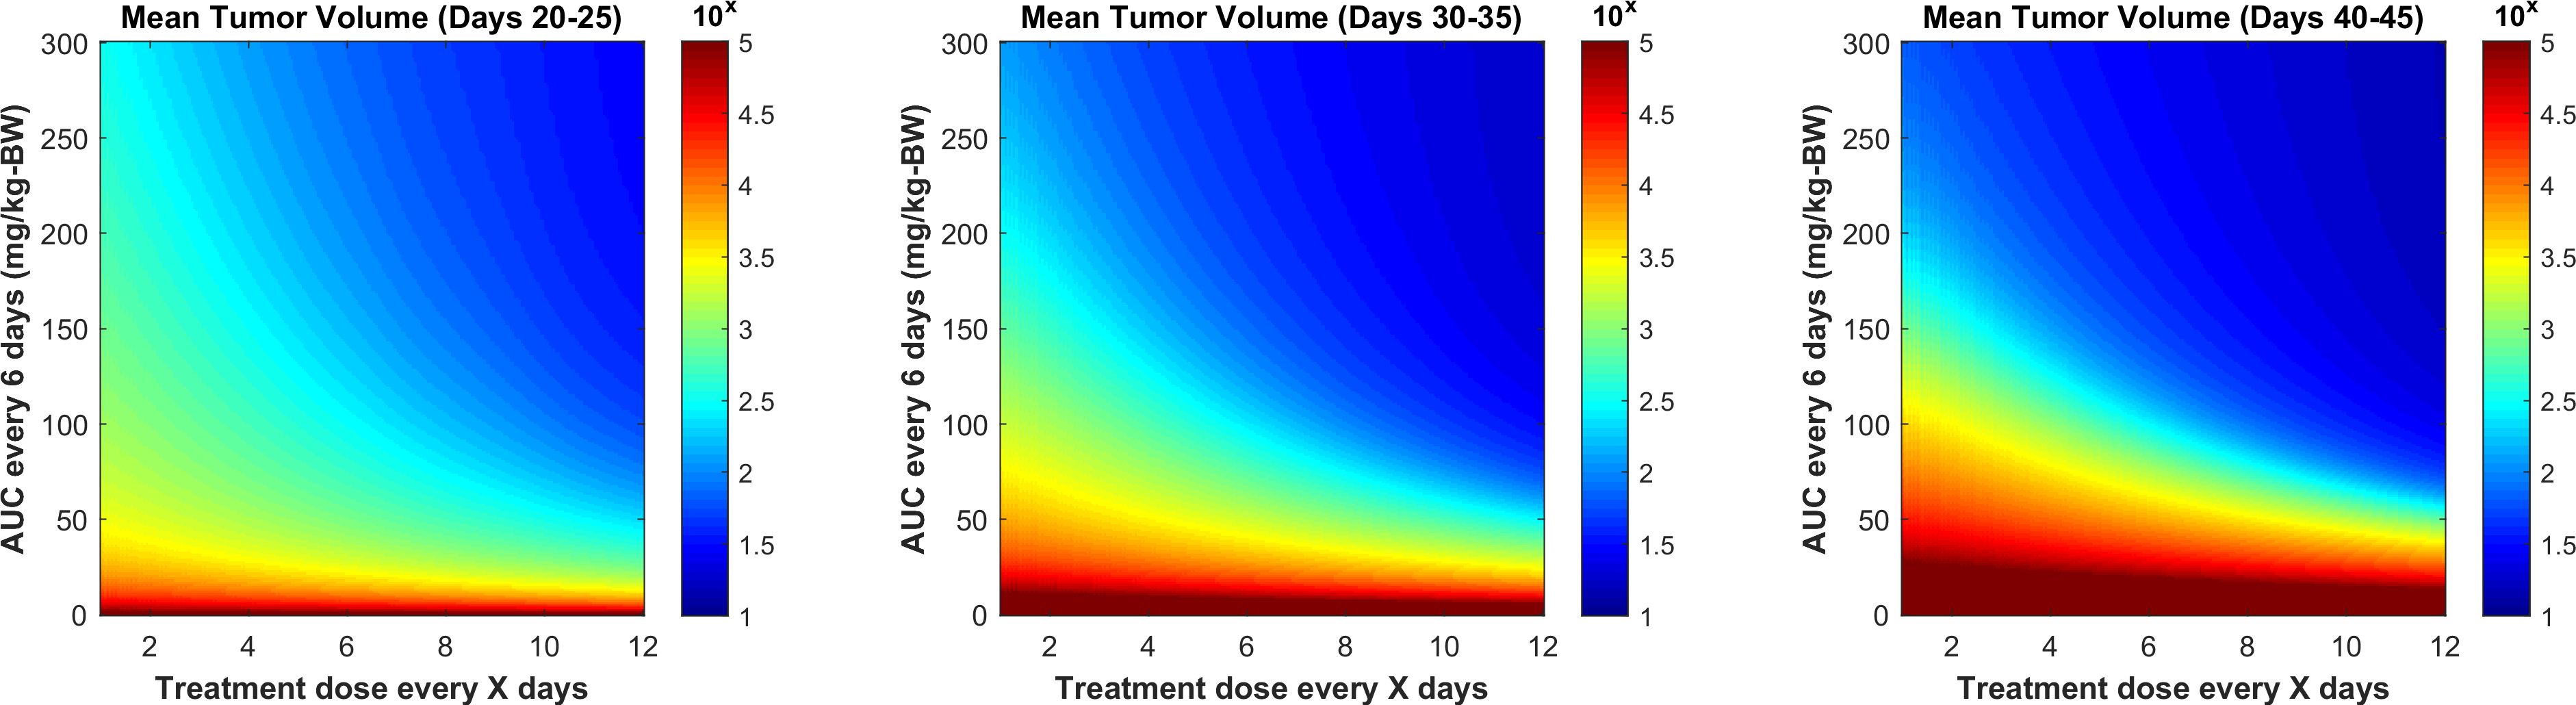
\includegraphics[width=1\linewidth]{chemo-metronomic.png} \\
	\vspace{0.5cm}
	The average tumor volume at different time ranges of 20-25 days (left), 30-35 days (middle), and 40-45 days (right) after starting a metronomic regimens. The horizontal axis represent the number of dose between each dose, y axis is the total amount of drug given to the animal every 6 days.
\end{frame}

\subsection{Optimal control}
\begin{frame}{Optimal control problem setup}
	Numerical software GPOPS\textunderscore II is used to solve the following setup for the optimal control problem.\\
	\begin{subequations}
	\begin{align}  \label{eq:ocp}
			\min_{u(t)} & \quad T(t_f), \\
			s.t. & \quad 
			\begin{bmatrix}
				0 \\ 0 \\ 0 \\ 0 \\ 0 \\ 0
			\end{bmatrix} 
			\leq
			\begin{bmatrix}
				C(t) \\ T(t) \\ I(t) \\ X(t) \\ Y(t) \\ u(t)
			\end{bmatrix}
			\leq
			\begin{bmatrix}
				C_m \\ T_m \\ I_m \\ X_m \\ Y_m \\ u_m
			\end{bmatrix},
			\\
			& \quad \int_0^{t_f} u(t) dt \leq U_m.
	\end{align}
	\end{subequations}
\end{frame}

\begin{frame}{Numerical result for a low input upper bound}
	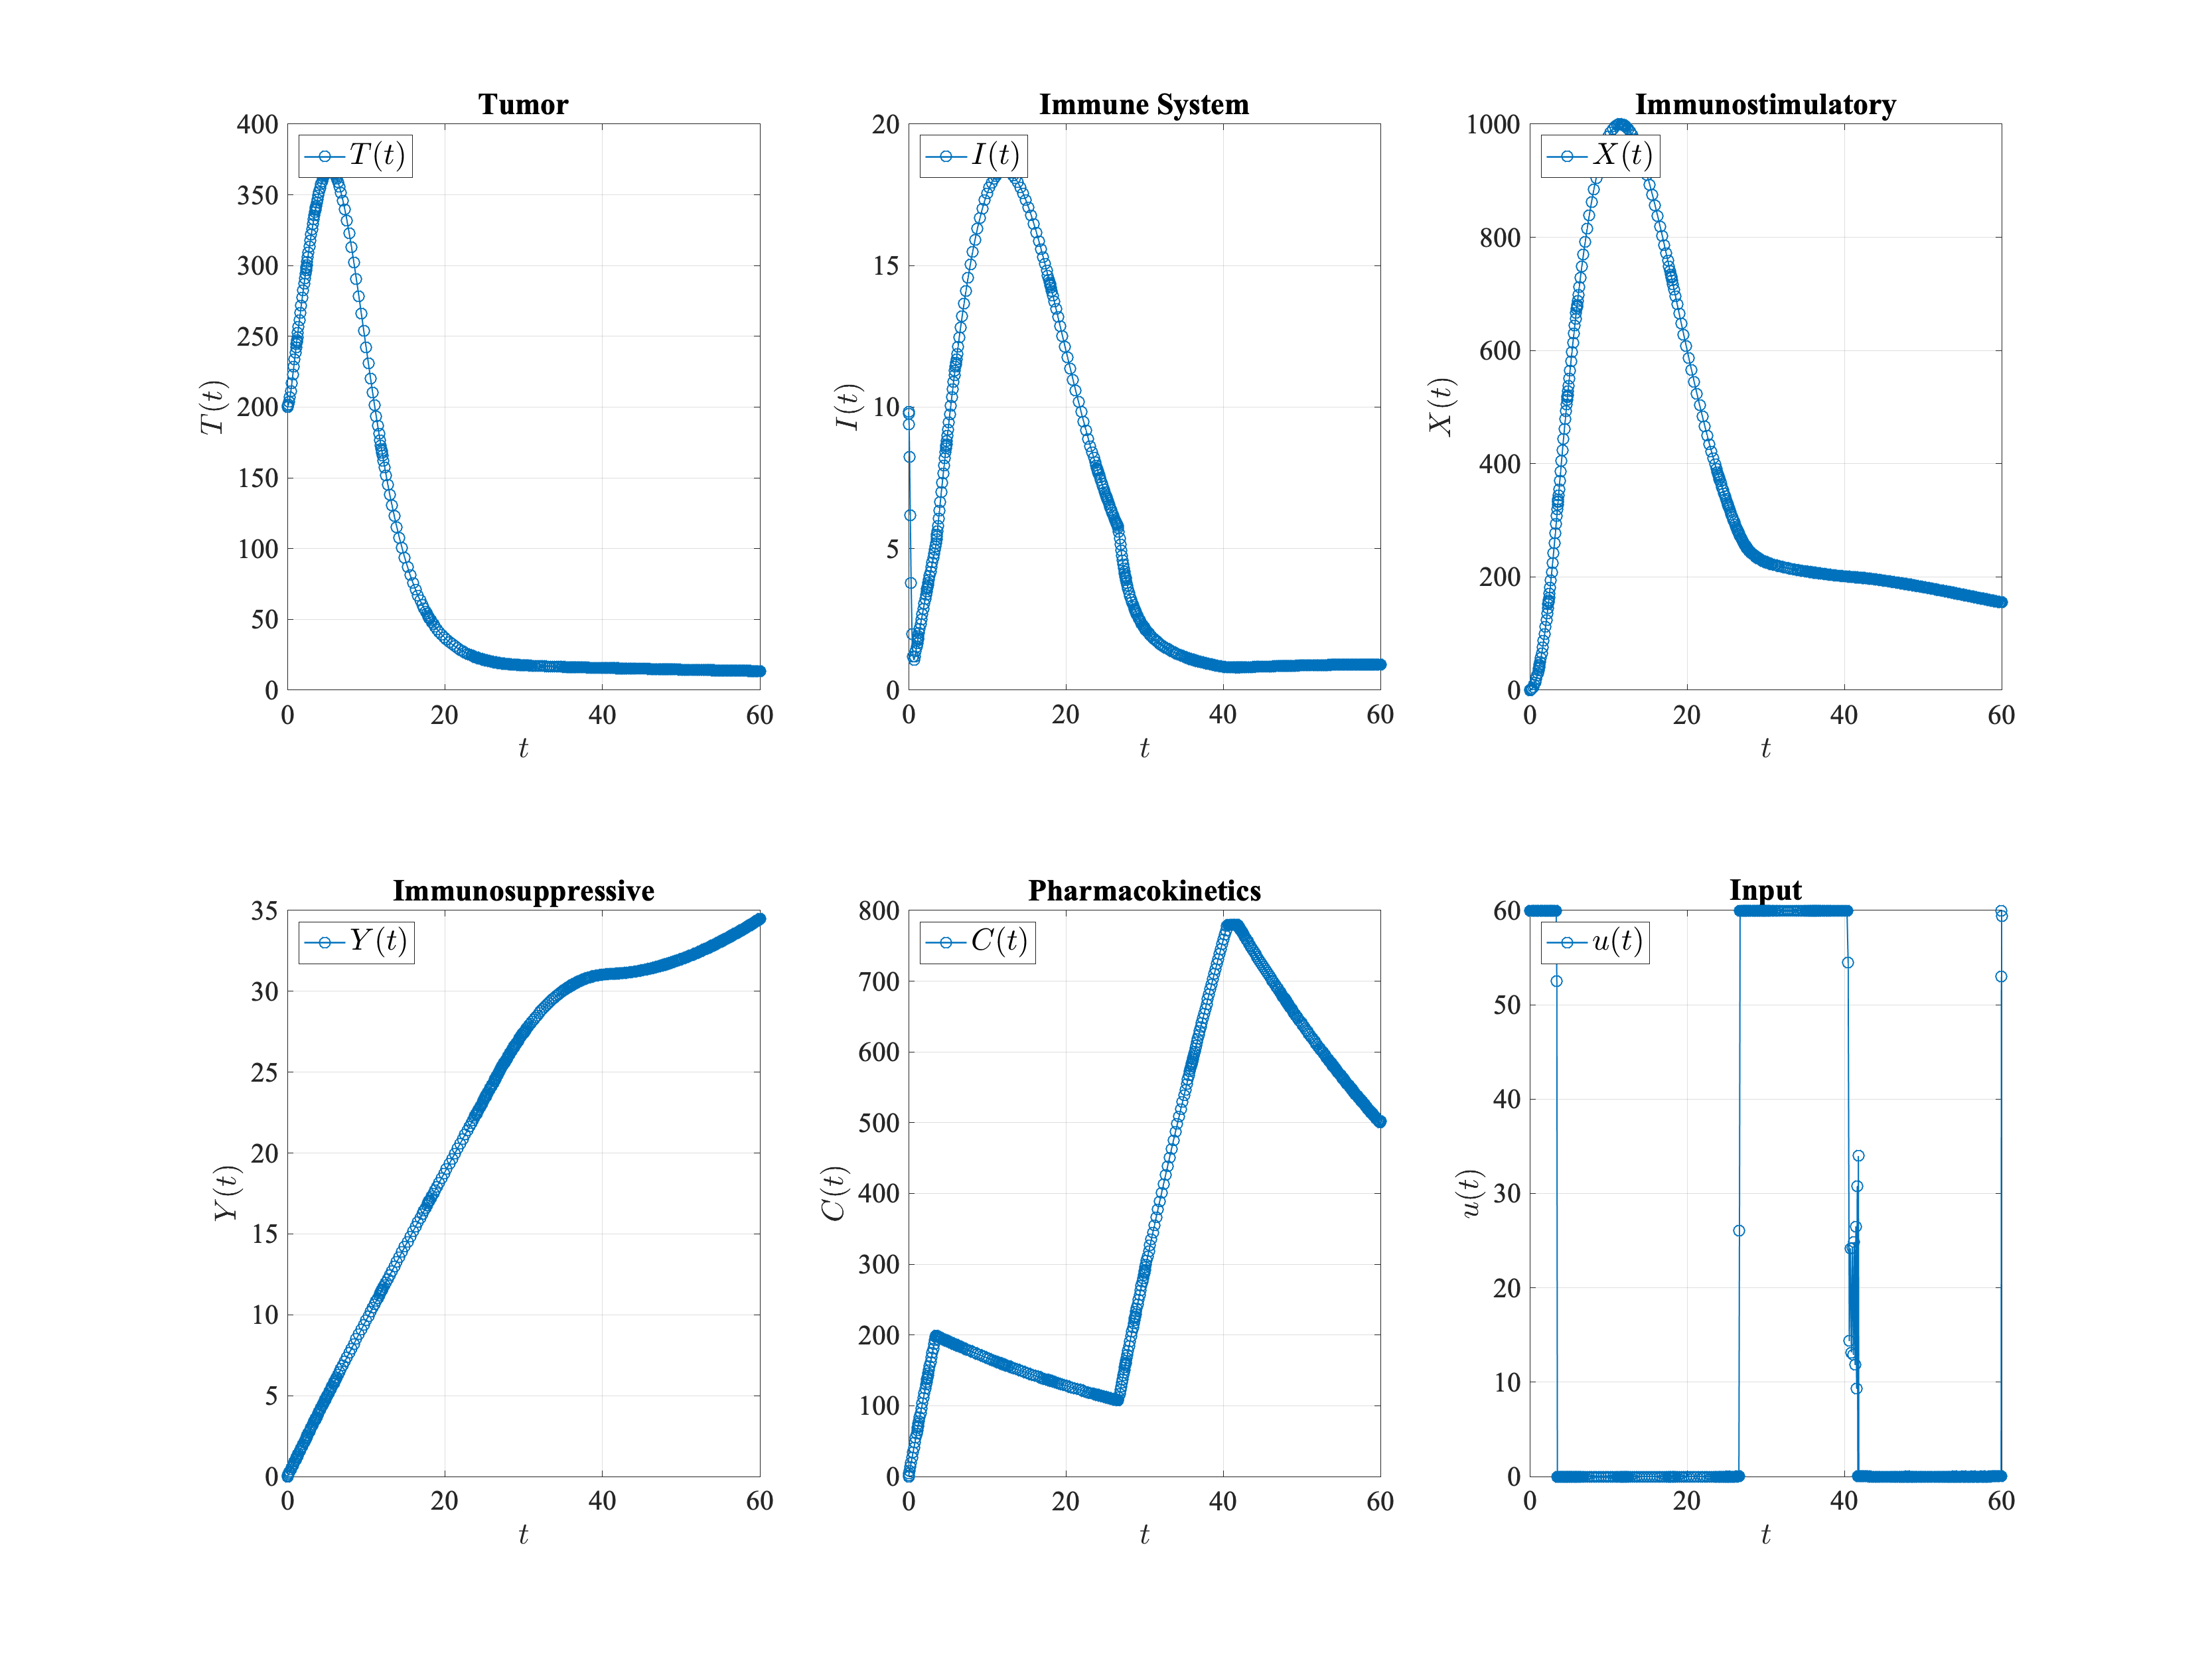
\includegraphics[width=1\linewidth]{chemo-optimalcontrol1.png} \\
	Circles show the final collocation points.
\end{frame}

\begin{frame}{Numerical result for a high input upper bound}
	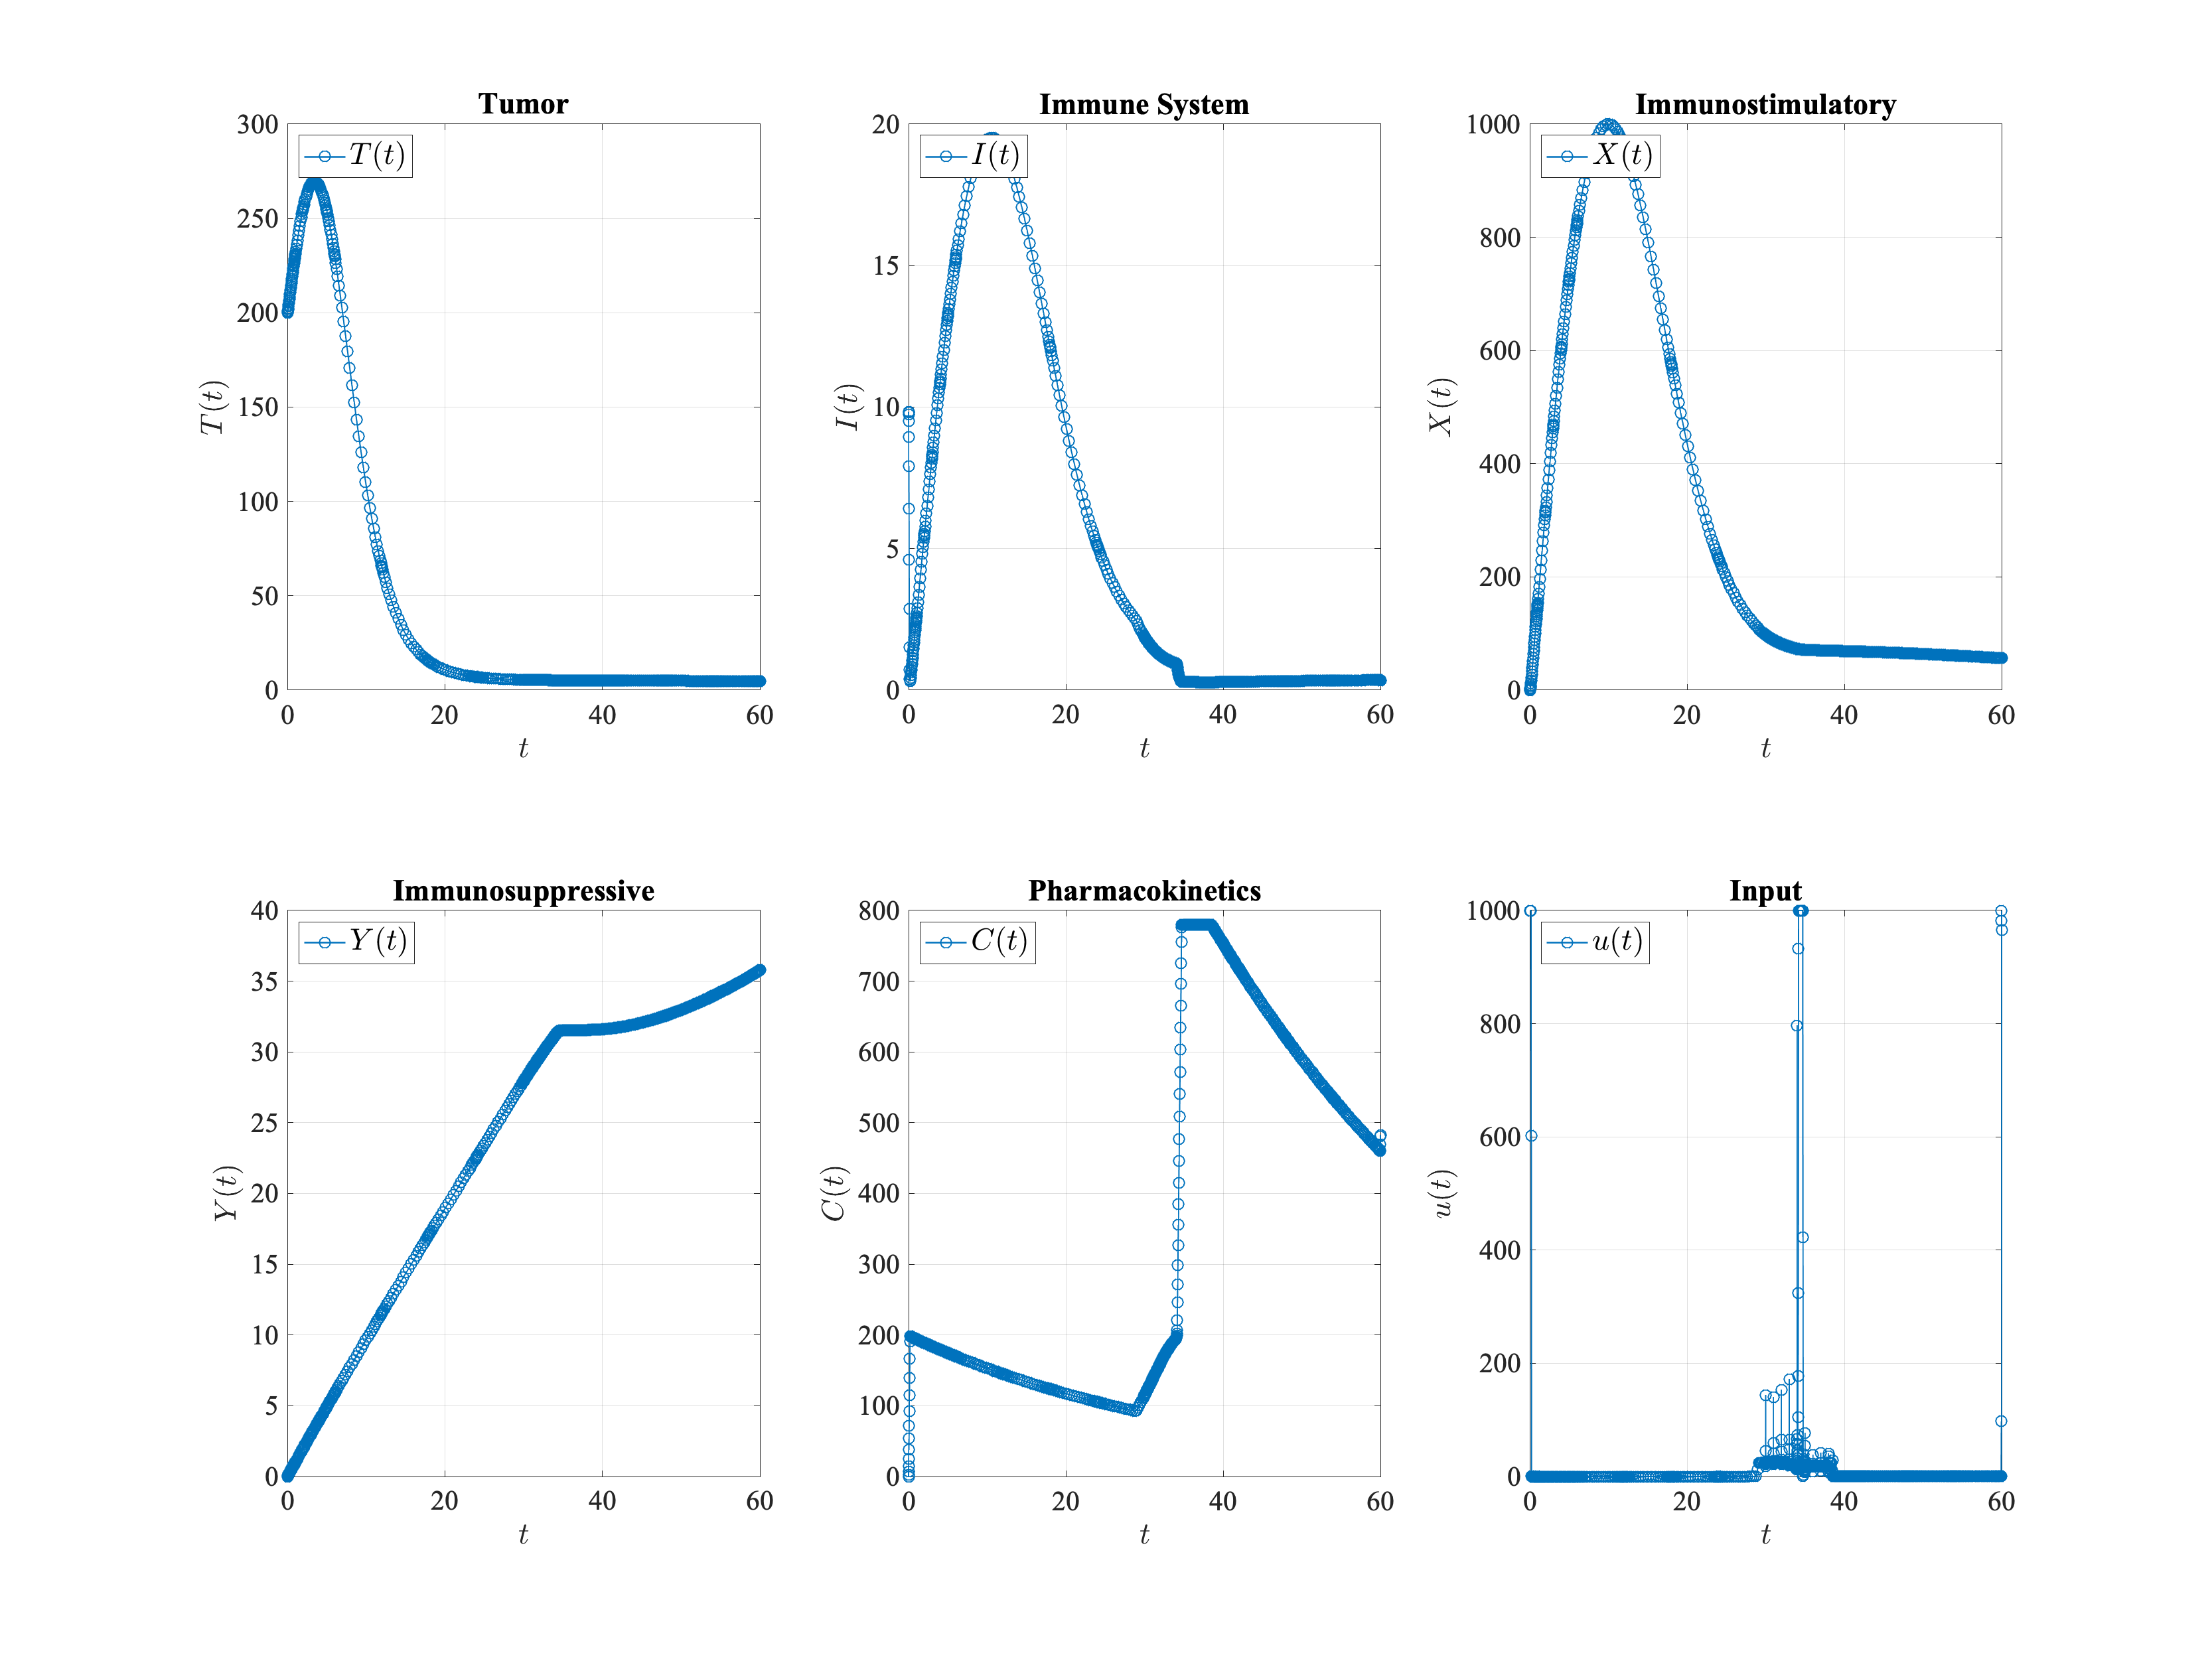
\includegraphics[width=1\linewidth]{chemo-optimalcontrol2.png} \\
	Circles show the final collocation points.
\end{frame}

\subsection{MDOR}
\begin{frame}{Optimal control vs. metronomic regimen}
	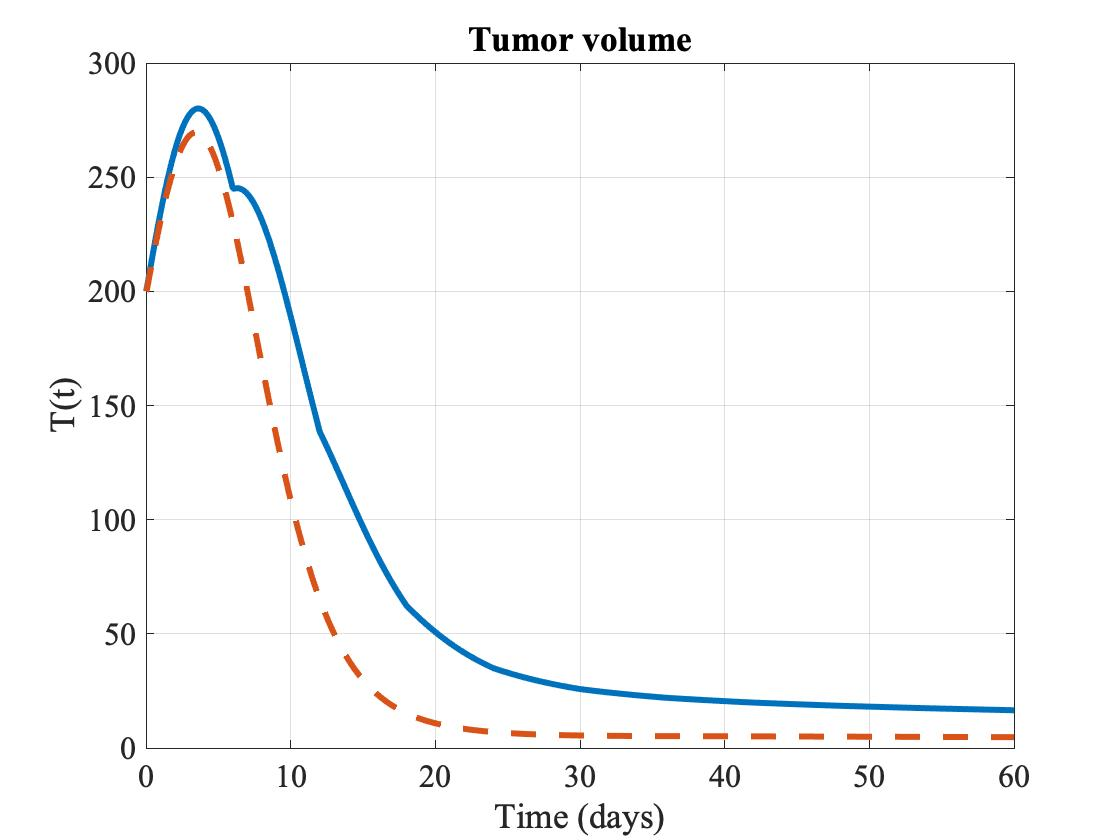
\includegraphics[width=0.49\textwidth]{chemo-comparison-oc1.jpeg}
	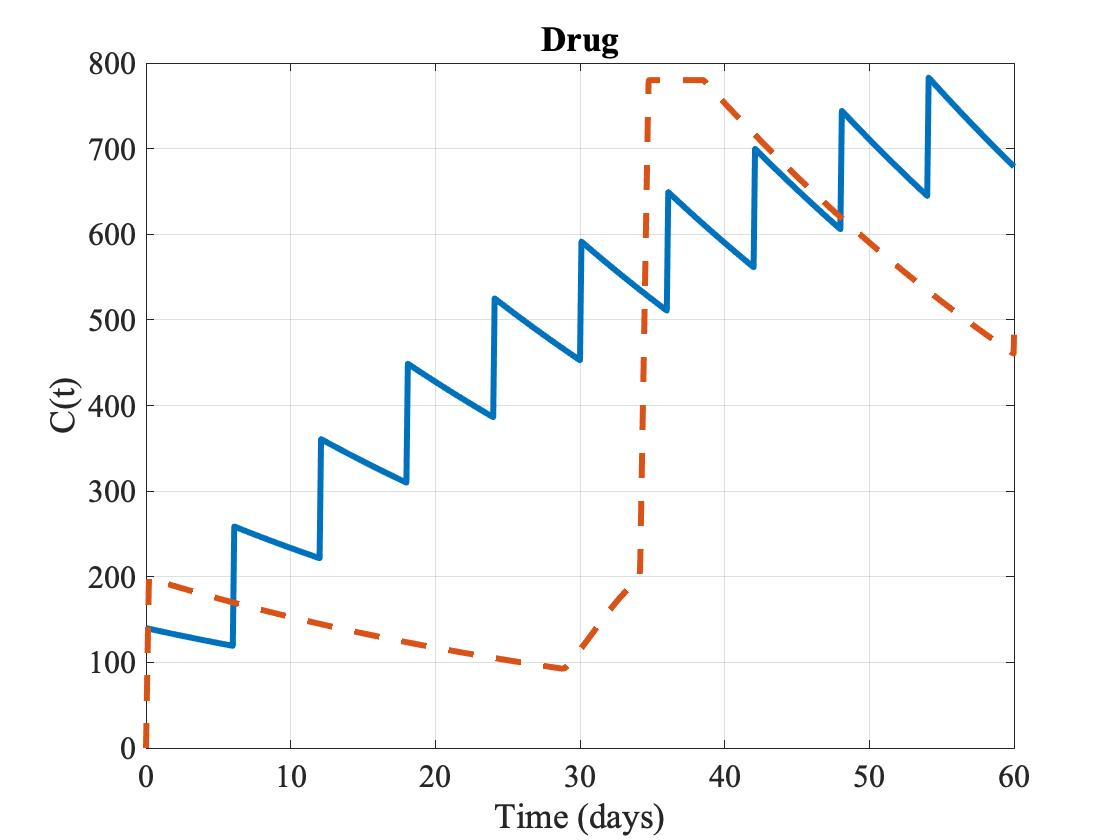
\includegraphics[width=0.49\textwidth]{chemo-comparison-oc2.jpeg} \\
	Comparing a standard 140 mg/kg Q6D metronomic chemotherapy plan (solid lines) with the obtained optimal control (dashed lines). \\ \vspace{0.5cm}
	However, The maximum tolerated dose is 300 mg/kg/day for CPA.
\end{frame}

\begin{frame}{Mathematically derived optimal regiment}
	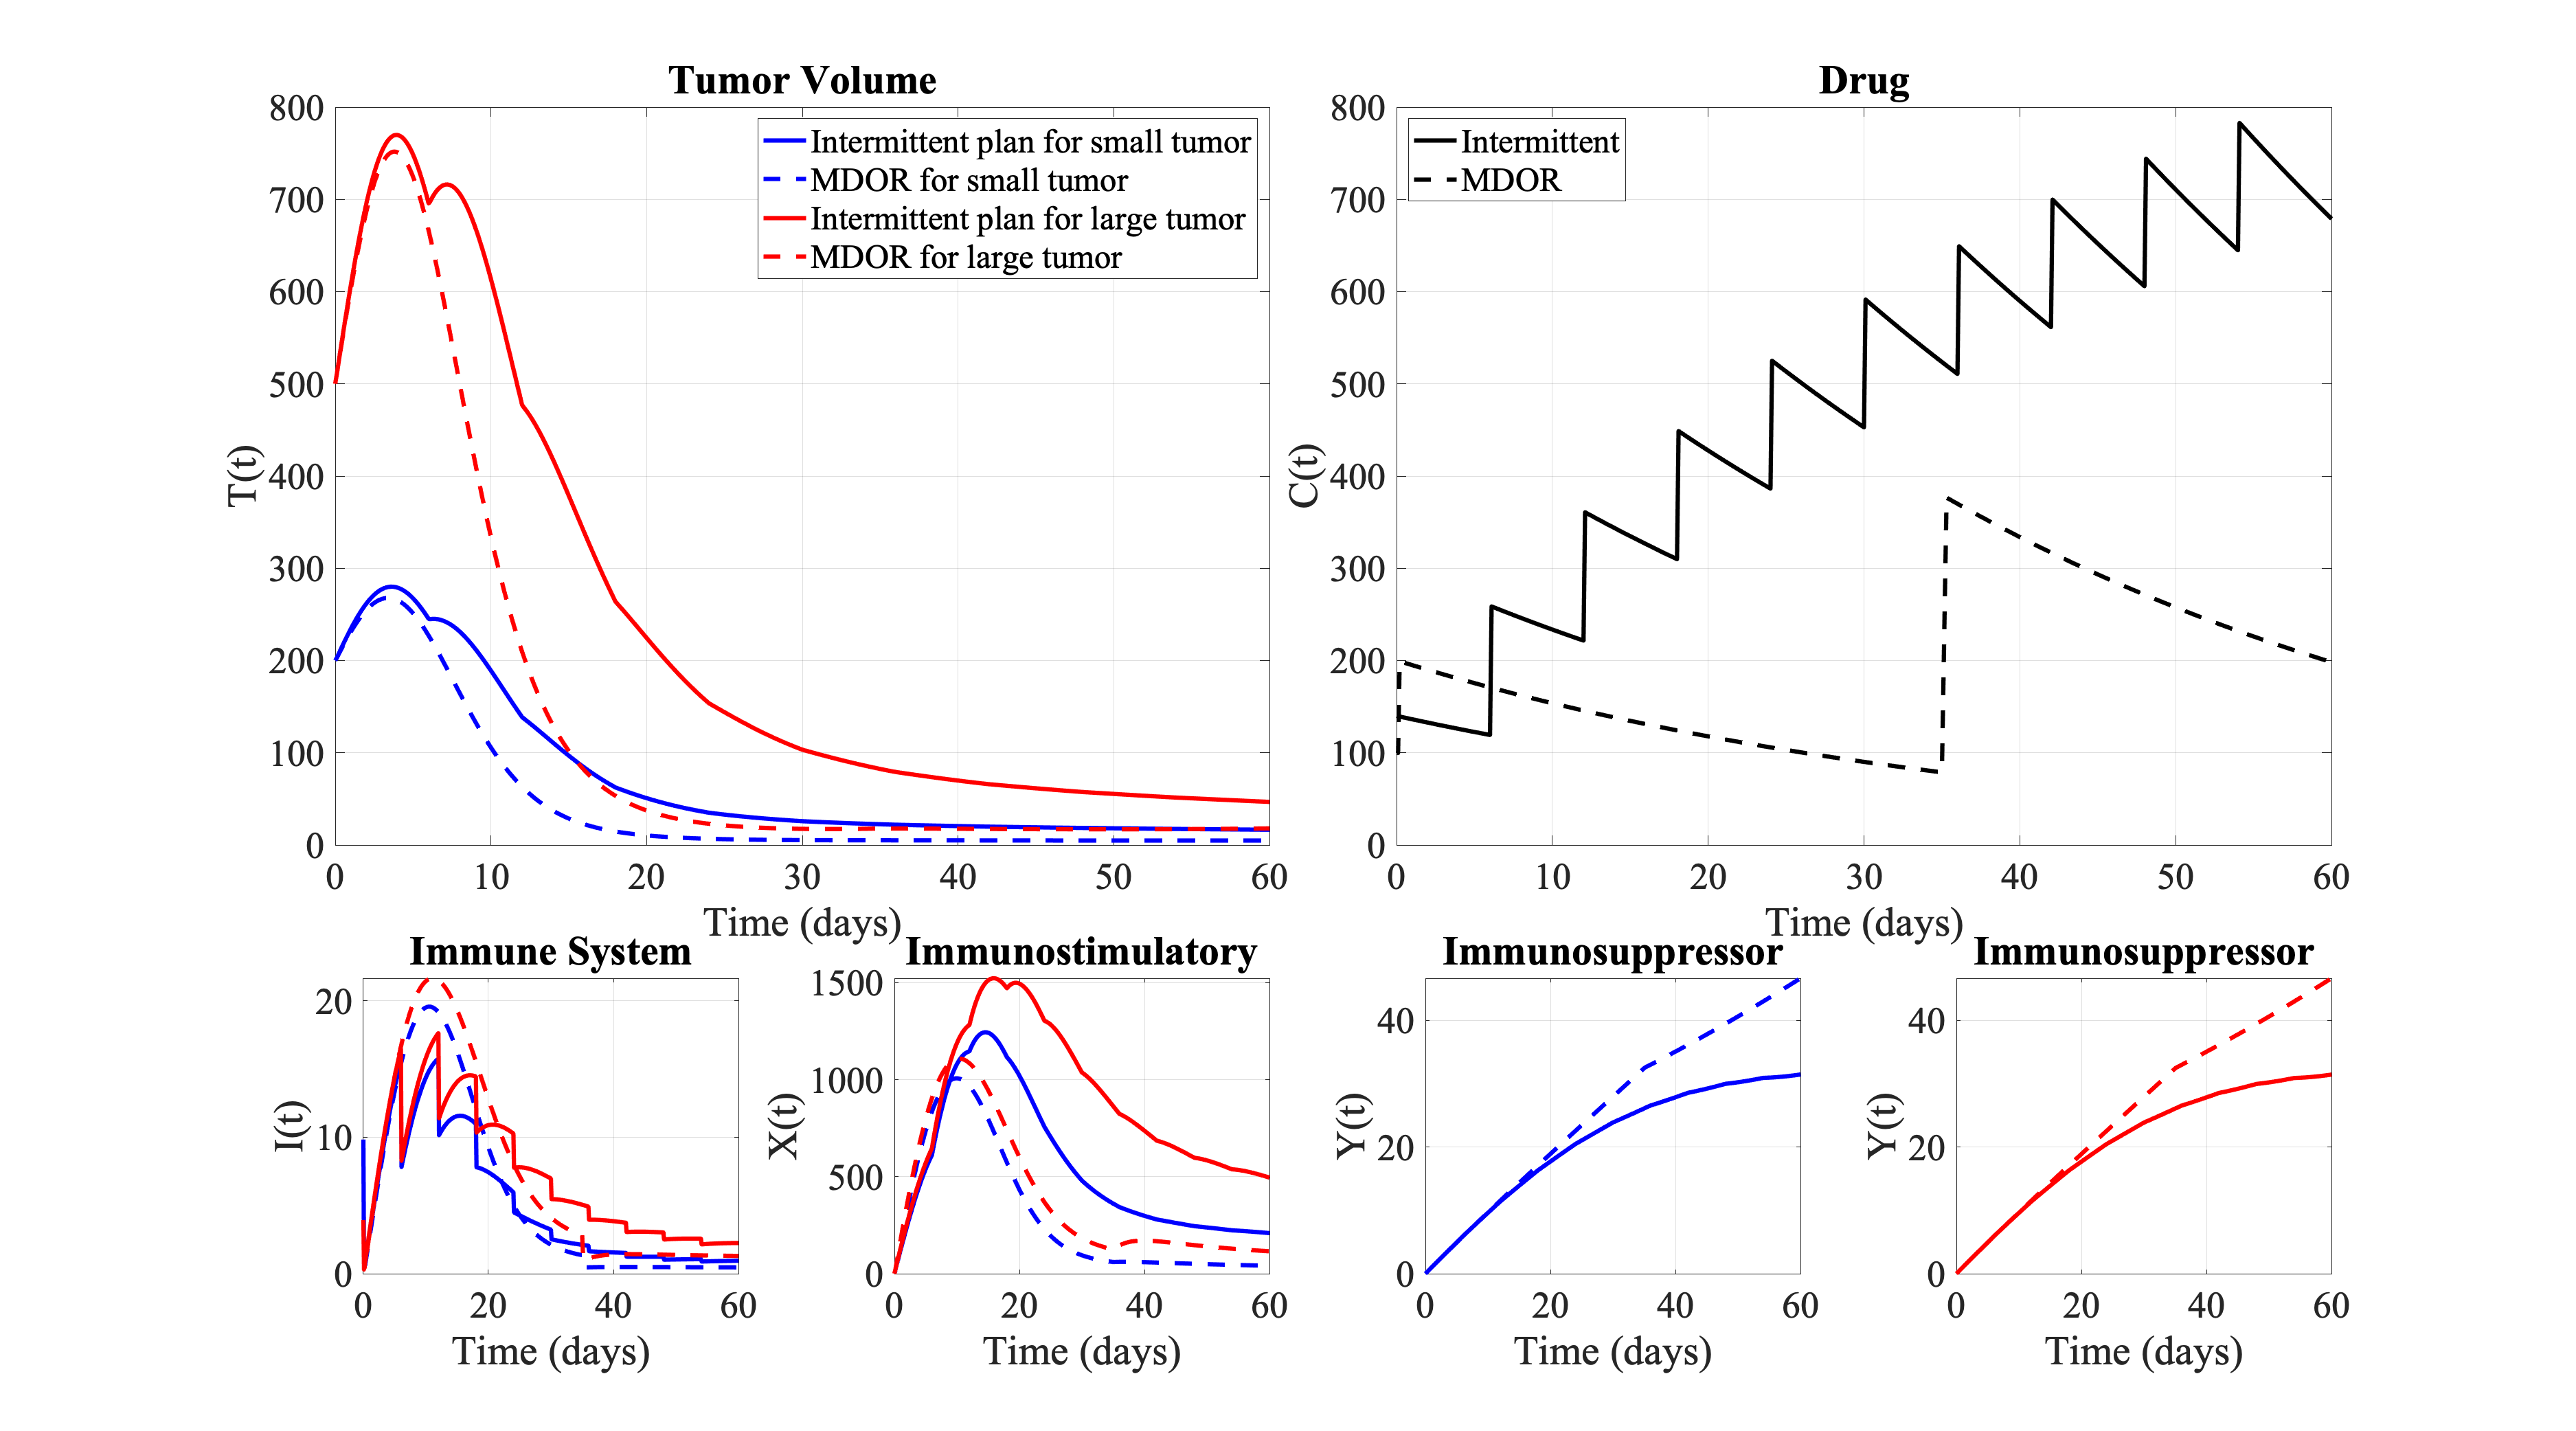
\includegraphics[width=1\textwidth]{chemo-final.png} \\
	Comparing a standard 140 mg/kg Q6D metronomic/intermittent plan (solid lines) and the mathematically derived optimal regimen (dashed lines). 
\end{frame}

\begin{frame}{A new viable regimen to be tested experimentally}
	\hspace{1cm}
	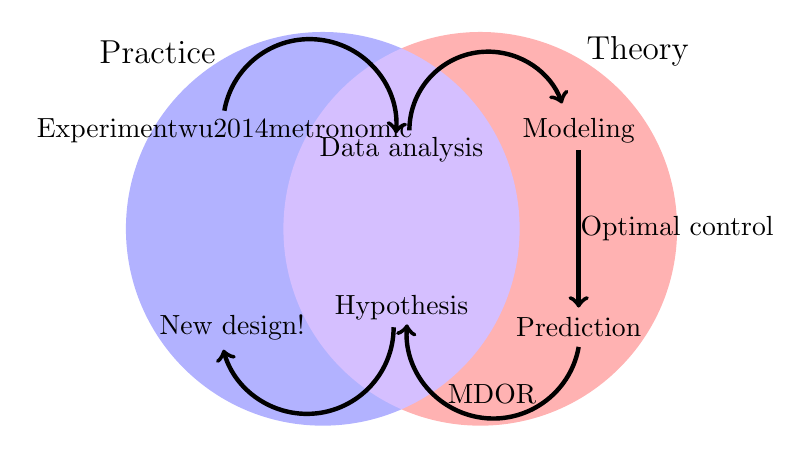
\begin{tikzpicture}
		\pgftransformscale{\myscalefactor}
		\begin{scope}[blend group = soft light]
			\fill[blue!30!white] (-2,0) ellipse (5 and 5);
			\fill[red!30!white]  (+2,0) ellipse (5 and 5);
		\end{scope}
		\draw[ultra thick, ->] (0.2,2.5) arc (0:-160:-2);
		\draw[ultra thick, ->] (-4.5,+3) arc (-10:-185:-2.2);
		\draw[ultra thick, ->] (-0.2,-2.5) arc (0:-165:+2.2);
		\draw[ultra thick, ->] (4.5,-3) arc (-10:-185:2.2);
%		\draw [ultra thick, ->] (-0.2,+1.5) -- (-0.2,-1.5);
%		\draw [ultra thick, ->] (+0.2,-1.5) -- (+0.2,+1.5);
		\draw [ultra thick, ->] (4.5,+2) -- (4.5,-2);
%		\draw [ultra thick, ->] (-4.5,-2) -- (-4.5,+2);
		\node at (0,+2) {Data analysis};
		\node at (4.5,+2.5)  {Modeling};
		\node at (7,+0.0)  {Optimal control};
		\node at (2.3,-4.2)  {MDOR};
		\node at (4.5,-2.5)  {Prediction};
		\node at (0,-2)  {Hypothesis};
		\node at (-4.5,+2.5)  {Experiment\footfullcite{wu2014metronomic}};
		\node at (-4.3,-2.5) {New design!};
		\node at (-6.2,4.5)[font=\large]    {Practice};
		\node at (+6,4.5)[font=\large]    {Theory};
	\end{tikzpicture}
\end{frame}

%-------------------------------------------------%
\section{Epidemic}

\begin{frame}{Social distancing (SD) in epidemics}
	During the COVID-19 epidemic, social distancing as a form of non-pharmaceutical intervention has been enacted in the US and other countries.
	\vspace{1cm}
	\begin{itemize}
		\item Motivation: Shortening the period of time that populations are socially distanced is economically advantageous.  
		\vspace{0.5cm}
		\item Objective: To reduce the disease burden (here measured as the peak of the infected population) while simultaneously minimizing the length of time that the population is socially distanced.  
	\end{itemize}
\end{frame}

\begin{frame}{Early days and limited data!}
	\vspace{0.5cm}
	\hspace{1cm}
	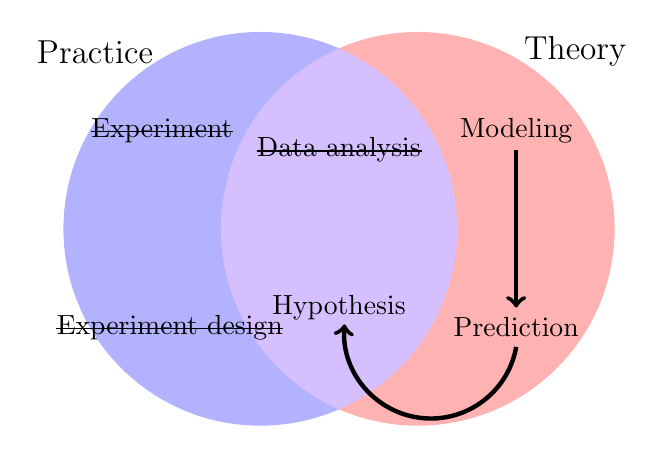
\begin{tikzpicture}
		\pgftransformscale{\myscalefactor}
		\begin{scope}[blend group = soft light]
			\fill[blue!30!white] (-2,0) ellipse (5 and 5);
			\fill[red!30!white]  (+2,0) ellipse (5 and 5);
		\end{scope}
%		\draw[ultra thick, ->] (0.2,2.5) arc (0:-160:-2);
%		\draw[ultra thick, ->] (-4.5,+3) arc (-10:-185:-2.2);
%		\draw[ultra thick, ->] (-0.2,-2.5) arc (0:-165:+2.2);
		\draw[ultra thick, ->] (4.5,-3) arc (-10:-185:2.2);
%		\draw [ultra thick, ->] (-0.2,+1.5) -- (-0.2,-1.5);
%		\draw [ultra thick, ->] (+0.2,-1.5) -- (+0.2,+1.5);
		\draw [ultra thick, ->] (4.5,+2) -- (4.5,-2);
%		\draw [ultra thick, ->] (-4.5,-2) -- (-4.5,+2);
		\node at (0,+2) {\st{Data analysis}};
		\node at (4.5,+2.5)  {Modeling};
		\node at (4.5,-2.5)  {Prediction};
		\node at (0,-2)  {Hypothesis};
		\node at (-4.5,+2.5)  {\st{Experiment}};
		\node at (-4.3,-2.5) {\st{Experiment design}};
		\node at (-6.2,4.5)[font=\large]    {Practice};
		\node at (+6,4.5)[font=\large]    {Theory};
	\end{tikzpicture}
\end{frame}

\subsection{Singel interval SD}

\begin{frame}{Mathematical model for a single interval SD}
	Assuming that $\beta$, the disease transmission rate, can be effectively reduced from $\beta_{n}$ (contact rate during normal time for non-distanced population) to $\beta_{d}$ (contact rate during social distancing) during distancing. \\ \vspace{0.5cm}
	\begin{equation} \label{eq:beta}
		\beta(t) = \left\{
		\begin{matrix} 
			\beta_n & \qquad 0 \leq t_s \\ 
			\beta_d & \qquad t_s \leq t < t_s+t_d \\
			\beta_n  & \qquad t_s+t_d \leq t 
		\end{matrix}
		\right. .
	\end{equation} \\ \vspace{0.5cm}
	Normalized infected population in \textit{SIR} model, with no re-infection. \\
	\hspace{2cm} 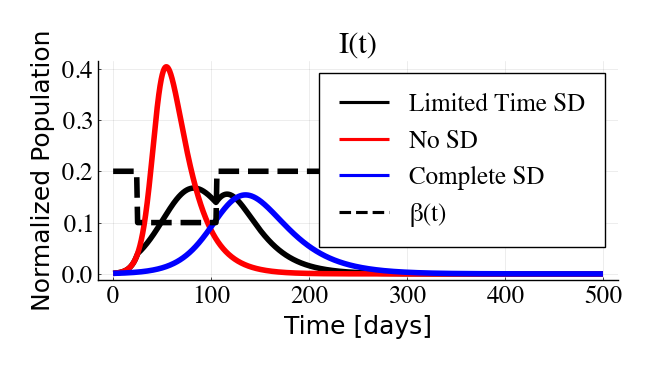
\includegraphics[width=0.6\textwidth]{epidemic-sd.png}\\
\end{frame}


%-------------------------------------------------%
\section{Acknowledgment}

\begin{frame}{This work is a result of teamwork}
	\small \hspace{1cm}
	{\begin{tabular}{r@{}l}
			Advisor:   \  & Eduardo Sontag \\ 
			Lab members:   \  & M. Ali Alradhawi, Anh Phong Tran, Zheming An, \\ 
			&  William Cho, Shu Wang, Tianchi Chen. \\ \\
			Presented & \, projects  \\ \\
			Chemotherapy: \  & Anh Phong Tran, Irina Kareva, M. Ali Alradhawi, \\ 
			& and Waxman Lab.\\
			Epidemics: \ & James Greene, M. Ali Alradhawi. \\ \\
			Other & \, projects  \\ \\
			\scriptsize Immunotherapy: \ & Irina Kareva, Kumpal Madrasi, Abed Alnaif, \\ & Anup Zutshi, and EMD Serono Inc team. \\ 
			\scriptsize Parkinson's Disease: \ & AMP-PD research community, and Sanofi team.  \\ 
			Ribosome: \ & M. Ali Alradhawi, Michael Margaliot, Nikolai Slavov, \\ & Edward Emmott. \\ \\
			Open-source & \, community: Julia team, Gleb Pogudin, Esteban Vargas.  \\
			& Bioconductor project.  \\
		\end{tabular}
	}
\end{frame}



%\begin{frame}
%	The basic definitions are from Miao et. al.~\footfullcite{miao2011identifiability}, for a general system:
%	
%	\begin{subequations}
%		\begin{align}
%			\dot x (t) &= f(t,x(t),u(t),\theta), \\
%			y(t) &= g(x(t), u(t), \theta).
%		\end{align}
%	\end{subequations}
%	
%	\begin{itemize}
%		\item $x(t) \in R^n$ is a vector of state variables.
%		\item $y(t) \in R^m$ is the measurement or output vector.
%		\item $u(t) \in R^p$ is the known system input vector.
%		\item $\theta \in R^q$ the parameter vector.
%		\item $\theta$ is unknown and has to be estimated based on experimental data. Here we assume that the parameters are constant.
%	\end{itemize}
%\end{frame}
%
%\subsection{Global identifiability}
%
%\begin{frame}{Global identifiabilty}
%	\begin{itemize}
%		\item \textbf{Definition: } A system structure is said to be globally identifiable if for any $\theta$ within an open neighborhood of some point $\theta^*$ in the parameter space, $y(u,\theta_1)=y(u,\theta_2)$ holds if and only if $\theta_1=\theta_2$.
%		\item \textbf{Example: } The following model is globally identifiable.
%			\begin{subequations} \label{eq:1}
%				\begin{align}
%					\dot x(t) &= a x(t) + b u(t), \\
%					y(t) &= x(t).
%				\end{align}
%			\end{subequations}
%		\item \textbf{Example: } The following model is not globally identifiable.
%		\begin{subequations} \label{eq:2}
%			\begin{align}
%				\dot x(t) &= \frac{a}{c} x(t) + b u(t), \\
%				y(t) &= x(t).
%			\end{align}
%		\end{subequations}
%		$y(t)$ of parameter sets $\theta_1=(a,b,c)= (1,2,3)$ and $\theta_2=(a,b,c)= (2,2,6)$ are the same.
%	\end{itemize}
%	
%\end{frame}
%
%\subsection{More definitions}
%
%\begin{frame}{More identifiabilty definitions}
%	\begin{itemize}
%		\item \textbf{Local identifiability: } A system structure is said to be locally identifiable if for any admissible input $u(t)$ and any two parameter vector $\theta_1$ and $\theta_2$ in the prameter space $\Theta$, $y(u,\theta_1) = y(u,\theta_2)$ holds if an only if $\theta_1=\theta_2$.
%		\item \textbf{Local strong identifiability } ($x_0$-identifiability). 
%		\item \textbf{Structural identifiability.} 
%		\item \textbf{Algebric identifiability.} 
%		\item \textbf{Algebric identifiability with known initial conditions.} 
%		\item \textbf{Structural equivalence: } Given two systems in the form
%		\begin{subequations}
%			\begin{align}
%				\dot x &= f(x(t,\theta)\theta) + u(t) g(x(t,\theta), \theta),\\
%				y &= h(x(t,\theta),\theta)
%			\end{align}
%		\end{subequations}
%		If there exist two parameters $\theta_1,\theta_2 \in \Theta$ such that, for the same admissible input $u(t)$, the solution of the two systems exists for $\theta_1$ and $\theta_2$, respectively, and the corresponding system outputs are the same, the system with parameters $\theta_1$ is said to be equivalent to the system with parameter $\theta_2$.
%	\end{itemize}
%	
%\end{frame}
%
%
%%-------------------------------------------------%
%\section{SIAN}
%
%%\begin{frame}{Structural Identifiability Analyzer (SIAN)\footfullcite{hong2019sian}}
%%	\begin{itemize}
%%		\item Open source structural identifiability software in Maple.
%%		\item Here is a benchmark for comparing SIAN performance with other available identifiability pacakges.
%%			\begin{figure}
%%				\includegraphics[width=1\linewidth]{sian-benchmark.png}
%%			\end{figure}
%%		\item A Maple app running SIAN online: \url{https://maple.cloud/app/6509768948056064}.
%%		\item A Julia package which often outperforms SIAN: \url{https://github.com/SciML/StructuralIdentifiability.jl}.
%%	\end{itemize}
%%\end{frame}
%
%
%\subsection{Basic examples}
%
%\begin{frame}[fragile]{Copy the following examples into Maple cloud app.}
%	Model \eqref{eq:1} where the parameters and initial conditions should be locally and globally identifiable:
%	\begin{lstlisting}
%		dx/dt = a*x + b*u(t)
%		y=x
%	\end{lstlisting}
%\vspace{20pt}
%	Model \eqref{eq:2} where $a$, and $c$ are not identifiable:
%	\begin{lstlisting}
%		dx/dt = a*x/c + b*u(t),
%		y=x
%	\end{lstlisting}
%\end{frame}
%
%\subsection{Tumor growth}
%
%\begin{frame}[fragile]{Tumor growth model~\footfullcite{simeoni2004predictive}.}
%	The minimal version of the tumor growth model with $n=2$:
%	\begin{subequations}
%		\begin{align}
%			\dot x_1(t) &= \frac{\lambda_0 x_1(t)}{(1+(\frac{\lambda_0 y(t)}{\lambda_1})^\Psi)^\frac{1}{\Psi}} - k_2 x_1(t) u(t), \\
%			\dot x_2(t) &= k_2 x_1(t) u(t) - k_1 x_2(t), \\
%			y(t) &= x_1(t) + x_2(t).
%		\end{align}
%	\end{subequations}
%	Let's try SIAN with the following code.
%	\begin{lstlisting}
%		dx1/dt = l0*x1/(1+(l0*y/l1)^P)^(1/P) - k2*x1*u(t),
%		dx2/dt = k2*x1*u(t) - k1*x2,
%		y = x1+x2
%	\end{lstlisting}
%	\color{red} error message:StringTools:-RegMatch. \\ 
%	\color{black} The solution is to use an equivalence form of the model. But why?
%	\begin{lstlisting}
%		dx1/dt = x1*w-k2*u(t)*x1, 
%		dx2/dt = k2*u(t)*x1-k1*x2,
%		dz/dt = psi*(x1*w-k1*x2)*z/y,
%		dw/dt = -(x1*w-k1*x2)*z*w/(y*(1+z)),
%		y= x1+x2
%	\end{lstlisting}
%\end{frame}
%
%\subsection{Parameter as power}
%
%\begin{frame}{In general, the algorithm does not allow noninteger powers and powers being parameters~\footnote{https://github.com/pogudingleb/SIAN/issues/2}}
%	
%	The solution is to define intermediate variables $z(t)$ and $w(t)$:
%	\begin{subequations}
%		\begin{align}
%			z(t) &= (\frac{\lambda_0 y(t)}{\lambda_1})^\Psi, \\
%			w(t) &= \frac{\lambda_0}{(1+z(t))^\frac{1}{\Psi}}.
%		\end{align}
%	\end{subequations}
%	Then dynamic can be rewritten in the following form.
%	\begin{subequations}
%		\begin{align}
%			\dot x_1(t) &= x_1(t) w(t) - k_2 u(t) x_1(t), \\
%			\dot x_2(t) &= k_2 u(t) x_1(t) - k_1 x_2(t), \\
%			\dot z(t) &=  \frac{\Psi z(t)}{y(t)} \dot y(t) = 
%			\frac{\Psi}{y(t)} (x_1(t) w(t) - k_1 x_2(t)), \\
%			\dot w(t) &= - \frac{w(t) \dot z(t)}{\Psi (1+z(t))} = 
%			- \frac{w(t) z(t)}{y(t) (1+z(t))} (x_1(t) w(t) - k_1 x_2(t)).
%		\end{align}
%	\end{subequations}
%\end{frame}
%
%%-------------------------------------------------%
%\section{Profile likelihood}
%
%\begin{frame}{Profile likelihood}
%	\begin{itemize}
%		\item Most useful to determine practical identifiability based on a given synthetic/expermental data.
%		\item Practical identifiability $\Rightarrow$ structural identifiabiility.
%		\item Structural identifiablity $\nRightarrow$ practical identifiablity.
%		\vspace{10pt}
%		\item An open source software in MATLAB~\footfullcite{raue2015data2dynamics}: 
%		\url{https://github.com/Data2Dynamics/d2d}.
%		\item An open source software in Python~\footfullcite{parra2020pdeparams}: \url{https://github.com/systemsmedicine/PDE_params}.
%	\end{itemize}
%\end{frame}
%
%\subsection{Basic examples}
%
%\begin{frame}
%	content...
%\end{frame}

\end{document}